\section{Задание 10}

Произвести фильтрацию одномерного процесса Орнштейна-Уленбека:
\begin{enumerate}
    \item Используя генератор белого шума, добавить случайную ошибку с 
    известной дисперсией к реализации процесса Орнштейна-Уленбека.
	\item При помощи одномерного фильтра Калмана оценить траекторию процесса по 
    зашумленному сигналу. Параметры процесса и белого шума считать известными.
	\item Рассмотреть случай, когда шум
	\begin{itemize}
		\item Является гауссовским.
		\item Имеет распределение Коши.
	\end{itemize}
\end{enumerate}
\bigskip

Белый шум для случайного процесса $x_{k+1} = A_k x_k$ будем моделировать 
линейным стохастическим уравнением 
\begin{equation} \label{white_noise}
	 x_{k+1} = A_k x_k + \omega_k,
\end{equation}
где $\omega_k$~--- случайная помеха, распределенная нормально или по Коши.

Фильтр Калмана для задачи \eqref{white_noise} имеет вид
\begin{equation} \label{kalman_filter}
    \left\{
    \begin{array}{lcr}
        \hat x_{k\mid k} = \hat x_{k\mid k-1} + R_{k \mid k-1} 
			C_k^T (C_k R_{k\mid k-1} C_k^T + N_k)^{-1} 
			(y_k - C_k \hat x_{k\mid k-1} - \Exp v_k),        	 			\\
		\hat x_{k+1\mid k} = A_k \hat x_{k\mid k} + \Exp \omega_k, 			\\
		R_{k\mid k} = R_{k\mid k-1} - R_{k\mid k-1} 
			C_k^T (C_k R_{k\mid k-1} C_k^T + N_k)^{-1} C_k R_{k\mid k-1},	\\
		R_{k+1 \mid k} = A_k R_{k\mid k} A_k^T + M_k,						\\
		\hat x_{0\mid -1} = \overline{x_0}, R_{0\mid -1} = s,				\\
    \end{array}
    \right.
\end{equation}
где  $y_k = C_k x_k + v_k$~--- измерения, 
$x_{k+1} = A_k x_k + \omega_k$~--- шаги. В случае процесса Орнштейна-Уленбека с 
параметрами $\lambda$, $\sigma$ система \eqref{kalman_filter} принимает вид
\begin{equation}
    \left\{
    \begin{array}{lcr}
        \hat x_{k\mid k} = \hat x_{k\mid k-1} + R_{k \mid k-1} 
			(R_{k\mid k-1} \sigma_v^2)^{-1} 
			(y_k - \hat x_{k\mid k-1}),										\\
		\hat x_{k+1\mid k} = e^{-\lambda\Delta t} \hat x_{k\mid k}, 		\\
		R_{k\mid k} = R_{k\mid k-1} - R_{k\mid k-1} 
			(R_{k\mid k-1} + \sigma_v^2)^{-1} R_{k\mid k-1},				\\
		R_{k+1 \mid k} = e^{-\lambda \Delta t} R_{k\mid k} A_k^T + 
		\sigma^2 (1-e^{-2\lambda \Delta t}),								\\
		\hat x_{0\mid -1} = 0, R_{0\mid -1} = \sigma^2,						\\
    \end{array}
    \right.
\end{equation}
Доверительный интервал фильтрации состовляет
\begin{equation}
	- k_{1-\frac{\alpha}{2}}\sqrt{R_{k\mid k}} < \hat x_{k\mid k} < 
	k_{1-\frac{\alpha}{2}}\sqrt{R_{k\mid k}},
\end{equation}
где $k_{1-\frac{\alpha}{2}}$~--- $(1-\frac{\alpha}{2})$-квантиль нормального 
распределения.

Пример работы программы см рис. \ref{filter}.

\begin{figure}[tbp]
	\centering
	\begin{subfigure}[b]{0.48\textwidth}
		\centering
		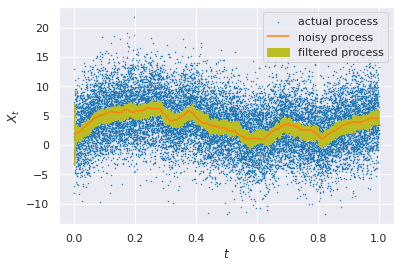
\includegraphics[width=\textwidth]{resources/task10_kalman_normal.png}
		\caption{Гауссовский шум}
	\end{subfigure}
	\hfill
	\begin{subfigure}[b]{0.48\textwidth}
		\centering
		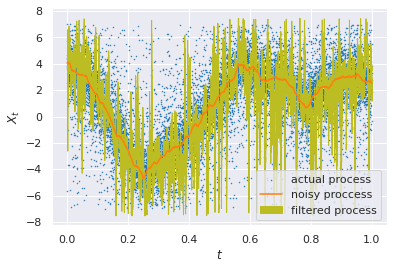
\includegraphics[width=\textwidth]{resources/task10_kalman_cauchy.png}
		\caption{Шум распределенный по Коши}
	\end{subfigure}
	\caption{Фильтрация Калмана}
	\label{filter}
\end{figure}
